\documentclass[../../main.tex]{subfiles}

\begin{document}

Im Kapitel über \emph{Abbildungen} hast du gelernt, dass sich Funktionen mithilfe von Graphen anschaulicher darstellen lassen. Vermutlich hast du aber keine wirkliche Vorstellung davon, wie der Graph einer Funktion aussieht, nur weil du die Abbildungsvorschrift kennst. Du hast schon gesehen, wie Nullstellen, Symmetrie und der Achsenabschnitt mit der Berechnungsvorschrift zusammenhängen:
\begin{itemize}
    \item für Nullstellen müssen Werte für $x$ gesucht werden, sodass $f(x)=0$ gilt
    \item für den Achsenabschnitt muss $f(0)$ berechnet werden
    \item für Symmetrie muss geprüft werden, ob $f(x)=f(-x)$ oder $f(x)=-f(-x)$ gilt
\end{itemize}
Während du die letzten beiden Punkte auch vor diesem Kapitel schon schnell überprüfen konntest, fehlte dir bisher ein Weg, systematisch Nullstellen zu bestimmen. Um für die Funktion $f(x)=3x-5$ die Nullstellen zu bestimmen, musst du herausfinden, wann $3x-5$ den Wert $0$ annimmt. Mit anderen Worten: Du musst eine Gleichung auflösen, nämlich $3x-5=0$. Das werden wir im Folgenden noch einmal genauer unter die Lupe nehmen, denn mit dem Wissen aus diesem Kapitel bist du mittlerweile in der Lage, lineare Gleichungen zu lösen.

\parpic[r]{
    \begin{tikzpicture}
        \begin{axis}[defgrid, domain=0:5, y=1cm, x=1cm, xtick={1,...,5}, ytick={1,2,3},ymin=0,ymax=3,xmin=0,xmax=5, samples=2]
            \addplot[color=violet] expression{0.3333333*x+0.33333333};
            \addplot[mark=*, only marks, fill=violet] coordinates {(2,1)};
            \addplot[mark=*, only marks, fill=violet] coordinates {(5,2)};
        \end{axis}
    \end{tikzpicture}
}

Wenn du von einer Funktion weißt, welche Nullstellen und welchen Achsenabschnitt sie hat, dann ist das natürlich ein guter Anfang. Aber diese Informationen verraten dir natürlich nur einen kleinen Teil vom Aussehen des Graphen. 
Wie sieht beispielsweise der Graph der Funktion $f(x)=3x-5$ aus und welche Abbildungsvorschrift hat eine Funktion, deren Graph die rechts abgebildete Gerade durch die Punkte $\coord{2}{1}$ und $\coord{5}{2}$ ist? Wann ist der Graph eine Gerade, wann ist er gebogen und wie steil ist er?

Die folgenden Abschnitte erklären, wie die Abbildungsvorschrift einer Funktion mit dem Aussehen ihres Graphen zusammenhängt -- also auch, welche Form er hat und wie steil er ist. Wir schauen uns in diesem Kapitel nur solche Funktionen an, bei denen sich diese Fragen mithilfe von linearen Gleichungen beantworten lassen. Die Kapitel über \emph{Quadratische Gleichungen} bzw. \emph{Differentialrechnung} bauen das hier präsentierte Wissen weiter aus.

\begin{center}
    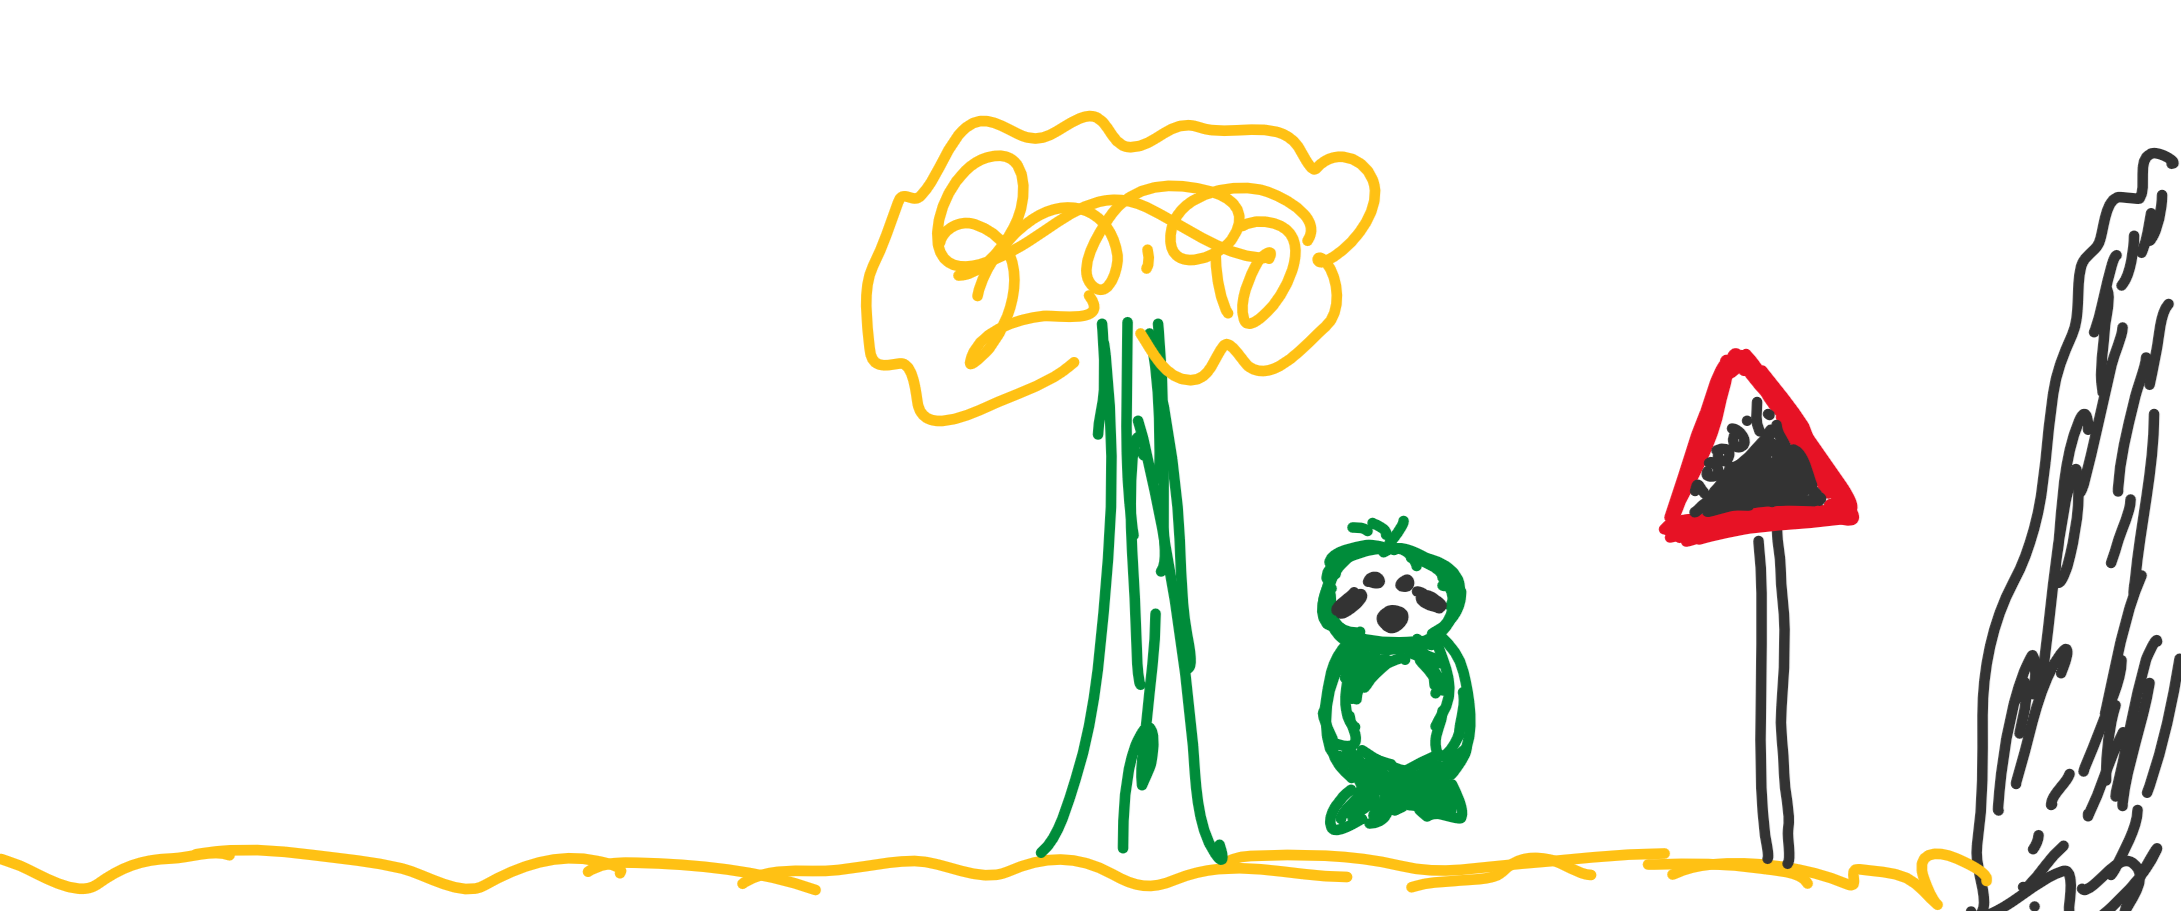
\includegraphics[height=4.7cm]{images/slope.png}
\end{center}

\subsection{Die Steigung einer Geraden}

\parpic[r]{
    \begin{tikzpicture}
        \begin{axis}[defgrid, domain=0:5, y=1cm, x=1cm, xtick={1,...,5}, ytick={1,2,3,4,5},ymin=0,ymax=5,xmin=0,xmax=5, samples=2]
            \addplot[color=orange] expression{x};
            \addplot[mark=*, only marks, fill=orange] coordinates {(1,1)};
            \draw[very thick,dashed,-latex] (1,1) -- (2,1) -- (2,2);
        \end{axis}
    \end{tikzpicture}
}
Eine wenig überraschende Eigenschaft von Geraden ist, dass sie immer in dieselbe Richtung führen. Sie biegen nicht zwischendurch ab und eine Gerade ist an jeder Stelle gleich steil.

Stelle dir also einmal vor, dass du auf der Geraden entlang gehst, und zwar immer in gleich großen Schritten nach rechts. Wenn du auf der Gerade auf der rechten Seite beim Punkt $\coord{1}{1}$ beginnst und der Gerade solange nach rechts folgst, bis du einen Schritt weiter rechts bist als zu Beginn, dann kommst du beim Punkt $\coord{2}{2}$ an. Während eines Schritts nach rechts hat sich die $y$-Koordinate also um $1$ vergrößert.

Weil Geraden an jeder Stelle in die gleiche Richtung führen, sind sie natürlich auch an jeder Stelle gleich steil. Wenn du also weiter rechts auf der Gerade angefangen hättest und einen Schritt nach rechts gegangen wärst, dann wärst du trotzdem genauso weit nach oben gekommen: Ebenfalls einen Schritt. Bei Geraden ist es also egal, wo du anfängst: Die Anzahl der Schritte nach oben pro Schritt nach rechts ist immer gleich.

\begin{example}[ex:slope-always-equal]{}
    \parpic[r]{
        \begin{tikzpicture}
            \begin{axis}[defgrid, domain=0:5, y=1cm, x=1cm, xtick={1,...,5}, ytick={1,2,3},ymin=0,ymax=3,xmin=0,xmax=5, samples=2]
                \addplot[color=violet] expression{0.5*x};
                \addplot[mark=*, only marks, fill=violet] coordinates {(2,1)};
                \addplot[mark=*, only marks, fill=red] coordinates {(1,0.5)};
                \addplot[mark=*, only marks, fill=red] coordinates {(3,1.5)};
                \draw[very thick,dashed,-latex] (1,0.5) -- (2,0.5) -- (2,1);
                \draw[very thick,dashed,-latex] (2,1) -- (3,1) -- (3,1.5);
                \draw[very thick,dashed,-latex] (3,1.5) -- (4,1.5) -- (4,2);
            \end{axis}
        \end{tikzpicture}
    }
    Die rechts abgebildete Gerade ist nicht so steil wie die Gerade weiter oben auf dieser Seite. Wenn du vom violetten Punkt einen Schritt nach rechts gehst und schaust, wie stark die Gerade währenddessen angestiegen ist, dann siehst du, dass sie nur einen halben Schrit auf der $y$-Achse nach oben gekommen ist.
    
    \picskip{0}
    Allerdings passiert das gleiche auch, wenn du bei einem der roten Punkte anfängst -- oder ganz allgemein: egal, wo du anfängst. Jeder der drei eingezeichneten Pfeile führt erst einen Schritt nach rechts und dann einen halben Schritt nach oben.
\end{example}

Während die Gerade in Beispiel \ref{ex:slope-always-equal} bei jedem Schritt nach rechts nur um $\frac{1}{2}$ nach oben gestiegen ist, hat die orangefarbene Gerade dabei immer $1$ Schritt in $y$-Richtung zurückgelegt. Dass die orangefarbene Gerade pro Schritt nach rechts mehr Schritte nach oben zurücklegt, führt natürlich dazu, dass sie steiler ist.

Die Information, wie stark die Gerade pro Schritt nach rechts ansteigt, genügt, um genau zu wissen, wie steil eine Gerade ist. Die Pfeile, die wir oben in die Bilder eingezeichnet haben, bilden zusammen mit dem Graphen ein Dreieck. Mithilfe eines solchen Dreiecks können wir die Steigung des Graphen bestimmen. Deshalb heißen die Dreiecke, die wir eingezeichnet haben, \textbf{Steigungsdreiecke}. Unter der \textbf{Steigung} einer Gerade verstehen wir dann die Höhe eines solchen Dreiecks, wenn wir einen Schritt nach rechts gehen.

\begin{example}[ex:multiple-slope-examples]{}
    Die drei hier abgebildeten Geraden sind natürlich alle unterschiedlich steil: Die linke ist steiler als die mittlere und die rechte fällt sogar.
    \begin{multicols}{3}
        \begin{tikzpicture}
            \begin{axis}[defgrid, domain=0:3, y=1cm, x=1cm, xtick={1,...,3}, ytick={1,...,6},ymin=0,ymax=6,xmin=0,xmax=3, samples=2]
                \addplot[color=violet] expression{2*x};
                \addplot[mark=*, only marks, fill=violet] coordinates {(1,2)};
                \draw[very thick,dashed,-latex] (1,2) -- (2,2) -- (2,4);
            \end{axis}
        \end{tikzpicture}

        \begin{tikzpicture}
            \begin{axis}[defgrid, domain=0:3, y=1cm, x=1cm, xtick={1,...,3}, ytick={1,...,6},ymin=0,ymax=6,xmin=0,xmax=3, samples=2]
                \addplot[color=violet] expression{0.3333*x};
                \addplot[mark=*, only marks, fill=violet] coordinates {(1,0.33333)};
                \draw[very thick,dashed,-latex] (1,0.33333) -- (2,0.33333) -- (2,0.66667);
            \end{axis}
        \end{tikzpicture}

        \begin{tikzpicture}
            \begin{axis}[defgrid, domain=0:3, y=1cm, x=1cm, xtick={1,...,3}, ytick={1,...,6},ymin=0,ymax=6,xmin=0,xmax=3, samples=2]
                \addplot[color=violet] expression{5-1.5*x};
                \addplot[mark=*, only marks, fill=violet] coordinates {(1,3.5)};
                \draw[very thick,dashed,-latex] (1,3.5) -- (2,3.5) -- (2,2);
            \end{axis}
        \end{tikzpicture}
    \end{multicols}
    Mithilfe der eingezeichneten Steigungsdreiecke lässt sich nun genau angeben, \emph{wie} steil die Geraden jeweils sind: Das Steigungsdreieck der ersten Gerade hat eine Höhe von $2$, also hat die linke Gerade eine Steigung von $2$. Die mittlere Gerade hat eine Steigung von $\frac{1}{3}$. Am besten siehst du das daran, dass du drei Schritte nach rechts brauchst, um einen Schritt nach oben zu machen. Bei einem Schrit nach rechts geht es also nur $\frac{1}{3}$ Schritt nach oben.

    Das Steigungsdreieck der rechten Gerade hat zwar eine Höhe von $1.5$ bzw. $\frac{3}{2}$, aber die Gerade hat eine negative Steigung von $-\frac{3}{2}$, denn der Pfeil zeigt nach unten.
\end{example}

Jetzt, da du weißt, dass die Steigung jeder Geraden sich durch eine einzelne Zahl angeben lässt, liegt die Frage nahe, wie sich eine Gerade mit einer vorgegebenen Steigung durch eine Abbildungsvorschrift erzeugen lässt. Der Ausgangspunkt des Steigungsdreiecks hat jeweils eine bestimmte Koordinate $\coord{x}{y}$ und stellt die Abbildungsregel $f(x)=y$ dar. Wenn wir jetzt auf einer Geraden mit der Steigung $a$ einen Schritt nach rechts gehen, dann erhalten wir einen Punkt, der die $x$-Koordinate $x+1$ hat (einen Schritt weiter rechts) und die $y$-Koordinate $y+a$ ($a$ Schritte weiter oben). Insgesamt ergibt das den Punkt $\coord{x+1}{y+a}$. Wir wissen nun also, dass
\[f(x)=y~\text{und}~f(x+1)=y+a\]
gelten muss. Wenn wir auf der rechten Seite $y$ durch $f(x)$ ersetzen, dann sehen wir dass $f(x+1)=f(x)+a$ gelten muss.

Bei linearen Gleichungen durfte auf jeder Seite ein Term der Art $ax+b$ stehen (mit Zahlen $a,b\in\Real$). Tatsächlich können wir mit einem solchen Term genau das erreichen, was wir wollen. Schauen wir uns einmal an, was passiert, wenn wir eine Funktion $f(x)=ax+b$ haben und $f(x+1)$ ausrechnen. Es gilt:
\[f(x+1)=a\cdot (x+1)+b=ax+a+b=\colorobrace{ax+b}{f(x)}+a=f(x)+a.\]
Hier steht also genau dasselbe wie weiter oben. Eine Funktion $f$ mit der Berechnungsvorschrift $f(x)=ax+b$ hat also eine Steigung von $a$.

\begin{example}{}
    Die linke Gerade aus Beispiel \ref{ex:multiple-slope-examples} hat eine Steigung von $2$. Sie gehört zur Funktion $f$ mit $f(x)=2x$. Wir haben das Steigungsdreieck bei $x=1$ angesetzt. Da $f(1)=2\cdot 1=2$ gilt, hat der violette Punkt die Koordinate $\coord{1}{2}$.

    Schauen wir uns den Funktionswert einen Schritt weiter rechts an, dann erhalten wir 
    \[f(1+1)=f(2)=2\cdot 2=4.\]
    Damit haben wir $f(2)-f(1)=4-2=2$. Also ist die Gerade um $2$ Einheiten nach oben gestiegen, während wir einen Schritt nach rechts gegangen sind.
\end{example}

[Steigung legt Graph nicht eindeutig fest: Was ist mit Verschiebungen?]

Aus dem Kapitel über \emph{Abbildungen} weißt du bereits, dass der Achsenabschnitt einer Funktion die Zahl ist, die du erhältst, wenn du $f(0)$ ausrechnest. Für $f(x)=ax+b$ können wir $f(0)$ leicht ausrechnen. Es gilt
\[f(0)=a\cdot 0+b=b.\]
Die Funktion $f(x)=ax+b$ hat also den Achsenabschnitt $b$. Damit wissen wir jetzt genau, wie der Graph einer Funktion aussieht, die die Berechnungsvorschrift $f(x)=ax+b$ hat:
\begin{itemize}
    \item der Graph ist eine Gerade mit der Steigung $a$
    \item der Graph hat den Achsenabschnitt $b$
\end{itemize}

\begin{theorem}{Geradengleichungen}
    Der Graph einer Funktion $f(x)=ax+b$ ist eine Gerade mit der Steigung $a$ und dem Achsenabschnitt $b$.
\end{theorem}

\begin{example}{}
    \parpic[r]{
        \begin{tikzpicture}
            \begin{axis}[defgrid, domain=0:4, y=0.5cm, x=1cm, xtick={1,...,4}, ytick={-5,...,7},ymin=-5,ymax=7,xmin=0,xmax=4, samples=2]
                \addplot[color=violet] expression{3*x-5};
                \addplot[mark=*, only marks, fill=violet] coordinates {(0,-5)};
                \addplot[mark=*, only marks, fill=violet] coordinates {(1,-2)};
            \end{axis}
        \end{tikzpicture}
    }
    Zu Beginn dieses Abschnitts haben wir die Frage gestellt, wie der Graph der Funktion 
    \[f(x)=\tikzmarknode{slope3x5}{3}x\tikzmarknode{axis3x5}{-5}\] 
    aussieht. Bereits vor dem Lesen dieses Kapitels wusstest du, dass er die $y$-Achse im Punkt $\coord{0}{-5}$ schneidet, also den \textcolor{violet}{Achsenabschnitt} $-5$ hat, denn es gilt $f(0)=-5$.
    \tikz[overlay, remember picture]{
        \draw[maincolor] ($(slope3x5) + (-0.75ex,-1ex)$) -- ++ (1.5ex, 0) -- ++ (0,2ex) -- ++ (-1.5ex,0) -- cycle;
        \draw[violet] ($(axis3x5) + (-1.4ex,-1ex)$) -- ++ (2.8ex, 0) -- ++ (0,2ex) -- ++ (-2.8ex,0) -- cycle;
    }
    Jetzt bist du sogar in der Lage, den Graphen vollständig zu zeichnen. Es handelt sich nämlich um eine Gerade durch den Punkt $\coord{0}{-5}$, die eine \textcolor{maincolor}{Steigung} von $3$ hat, also pro Schritt nach rechts drei Schritte nach oben steigt.

    \picskip{1}
    Mithilfe dieser beiden Informationen (also Steigung und Achsenabschnitt) ist eindeutig festgelegt, dass die Gerade wie rechts abgebildet aussehen muss. Du kannst sie zeichnen, indem du beim Punkt auf der $y$-Achse beginnst, den du als Achsenabschnitt berechnet hast (linker violetter Punkt). Anschließend zeichnest du einen Punkt einen Schritt weiter rechts ein, der $3$ Schritte weiter oben liegt als der erste Punkt (denn $3$ ist die Steigung). Dann zeichnest du eine Gerade durch die beiden Punkte und erhältst den Graphen der Funktion $f$.
\end{example}

\subsection{Punkte auf Funktionsgeraden}

Nullstellen

Interpolation

\end{document}
